\section{Design Language}
The design language, which is also known as design vocabulary, is the design guidelines for \projectname{}. 
The objects here will have an important role in the systems user interface, and their design language is therefore described here.

\subsection{Color scheme}
\begin{figure}[htb]
    \centering
    
\includegraphics[width=\textwidth]{gfx/color_schema.pdf}
    \caption{color schema of \projectname{}.}
    \label{fig:color_schema}
\end{figure}

The color schema seen in \figref{fig:color_schema} shows the colors that are being used in the applications design. \fixme{hvorfor har vi valgt de farver fremfor orange og lyserød?}

\subsection{Fonts}
The family of fonts will be: Arial, Helvetica. 
These fonts have been selected because they are common both in Windows and Mac and therefore they are browser safe \cite{common_fonts}, meaning that the system will look the same no matter what operating system the user is using.

\subsection{Shapes}
All boxes that the user can interact with in the system, will be displayed with rounded corners.
This was done to make the interaction with the boxes as simple and straight forward as possible for the user.

\subsection{Layouts}
\begin{figure}[htb]
    \centering
    
\includegraphics[width=\textwidth]{gfx/menu.pdf}
    \caption{The menu of the application, with the control menu point activated.}
    \label{fig:menu_design}
\end{figure}

In \figref{fig:menu_design} the menu of the application is seen. 
In the figure, the bullet ``Control'' is active and therefore shown with a grey background color. 
All other menues have a black background color and are seperated with white spaces.

\begin{figure}[htb]
    \centering
    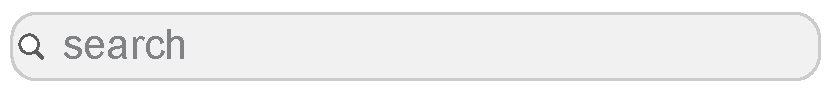
\includegraphics[width=\textwidth]{gfx/search.pdf}
    \caption{Search bar of the application}
    \label{fig:search_bar_design}
\end{figure}

In \figref{fig:search_bar_design} the search bar of the application is seen. 
The ``search'' text will disappear when the bare is clicked, and if the user types anything this will be shown in the search bar instead.

\begin{figure}[htb]
    \centering
    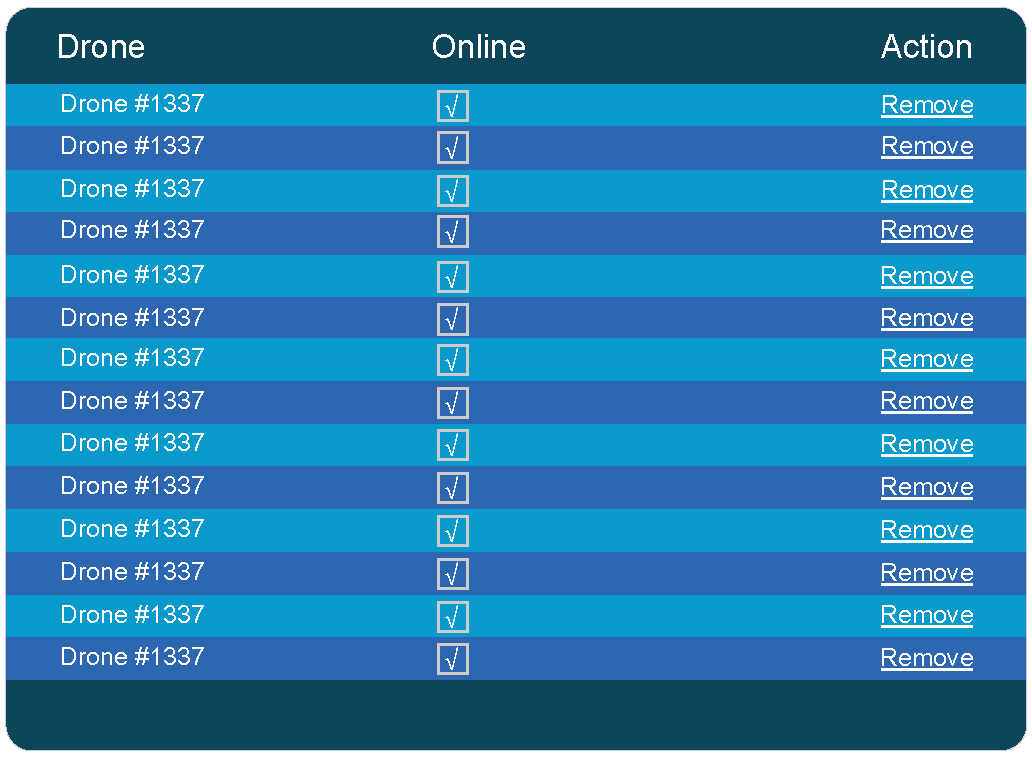
\includegraphics[width=\textwidth]{gfx/table.pdf}
    \caption{Table design for the application.}
    \label{fig:table_design}
\end{figure}
In \figref{fig:table_design} the general design for tables of the application is seen. 
Odd rows will be light blue and even rows will be blue.

\begin{figure}[htb]
    \centering
    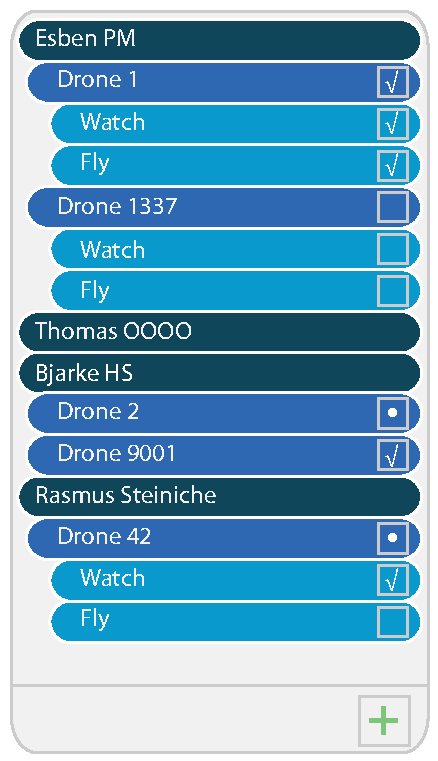
\includegraphics[scale=1.0]{gfx/list.pdf}
    \caption{List design for the application.}
    \label{fig:list_design}
\end{figure}
The list design seen in \figref{fig:list_design} is the core list item in the application. This list can show more and less information depending on where the user clicks. All levels are represented in \figref{fig:list_design} where a dark blue tab item with a name is a user in the system, the blue is a drone and the light blue is the privilege for the selected drone.
The list is made in such a way that the levels can be distinguished by the indent of the item.
The boxes in \figref{fig:list_design} shows the privilege status of an item. There are three different states these boxes can be in

\begin{itemize}
	\item Not marked
	\item Dotted
	\item ticked
\end{itemize}
 
If a box is not marked like ``Drone 1337'' the user have no privileges for this drone. If a box is dotted the user have some privileges for this drone like ``Drone 42''. If a box is ticked the user have all privileges for this drone e.g. Drone 1.

\begin{figure}[htb]
    \centering
    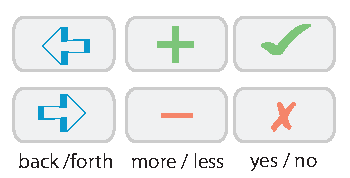
\includegraphics[scale=1.0]{gfx/button.pdf}
    \caption{Button design for the application.}
    \label{fig:button_design}
\end{figure}

The \projectname{} application have also gotten its own button design seen in \figref{fig:button_design}. There are three different groups of buttons and six buttons in total.
These buttons is used to navigate the site, make a selection for add or remove or accepting or declining depending on the situation.